\subsection*{Actividad 1.3}

Modelos de automóvil 1 y 2.

\begin{align*}
    D_1 & = t             &
    D_2 & = \frac{t^2}{2}
\end{align*}

\subsubsection*{Parte A}

\textbf{a)} Representación gráfica de los dos modelos.

\begin{center}
    \begin{tikzpicture}
        \begin{axis}[
                axis lines = left,
                xlabel = \(t\),
                ylabel = {\(D(t)\)},
                clip = false,
            ]
            % D_1
            \addplot [
                domain=0:10,
                samples=200,
                color=blue,
            ]
            {x};
            \addlegendentry{\(D_1=t\)}

            % D_2
            \addplot[
                domain=0:10,
                samples=200,
                color=red,
            ]
            {x*x/2};
            \addlegendentry{\(D_2=\frac{t^2}{2}\)}
        \end{axis}
    \end{tikzpicture}
\end{center}

\textbf{b)} Kilómetros recorridos al cabo de 1, 2 y 3 minutos.

\begin{center}
    \begin{tabular}{ c c c }
        t      & $D_1$ & $D_2$ \\
        \hline &               \\ [-1em]
        1      & 1     & $1/2$ \\
        2      & 2     & 2     \\
        3      & 3     & $9/2$ \\
        \hline
        \vspace{12pt}
    \end{tabular}
\end{center}

\textbf{c)} Velocidad media en intervalos [0, 1], [0, 2], [0, 3] y [1, 2].

\begin{center}
    \begin{tabular}{ c c c }
        Intervalo & $D_1$ & $D_2$ \\
        \hline    &               \\ [-1em]
        $[0, 1]$  & 1     & $1/2$ \\
        $[0, 2]$  & 1     & 1     \\
        $[0, 3]$  & 1     & $3/2$ \\
        $[1, 2]$  & 1     & $3/2$ \\
        \hline
    \end{tabular}
\end{center}

\textbf{Conclusiones.}
Observando la velocidad media del modelo 1 se puede notar que esta es constante para toda la trayectoria,
situación lo esperable en un modelo lineal.
Como la pendiente es constante,
el cambio en la distancia es proporcional al cambio en el tiempo.

La situación es diferente en el modelo 2.
Al tratase de un modelo cuadrático,
la velocidad media cambia según el período de tiempo considerado,
creciendo constantemente en función del tiempo.

Ello llevaría a concluir que uno de los automóviles se desplaza de manera uniforme,
mientras el otro lo hace de manera uniformemente variada.

\vspace{10pt}

\textbf{d)} Para calcular la velocidad en los minutos 1 y 2 recurrimos a la derivada de cada una de las funciones:

\begin{align*}
    D_1' & = 1 &
    D_2' & = t
\end{align*}

\begin{center}
    \begin{tabular}{ c c c }
        t      & $D'_1$ & $D'_2$ \\
        \hline &                 \\ [-1em]
        1      & 1      & 1      \\
        2      & 1      & 2      \\
        \hline
    \end{tabular}
\end{center}

\textbf{e)} Las tangentes a la distancia recorrida por el automóvil 2, en los puntos 1 y 2, son las siguientes:

\begin{center}
    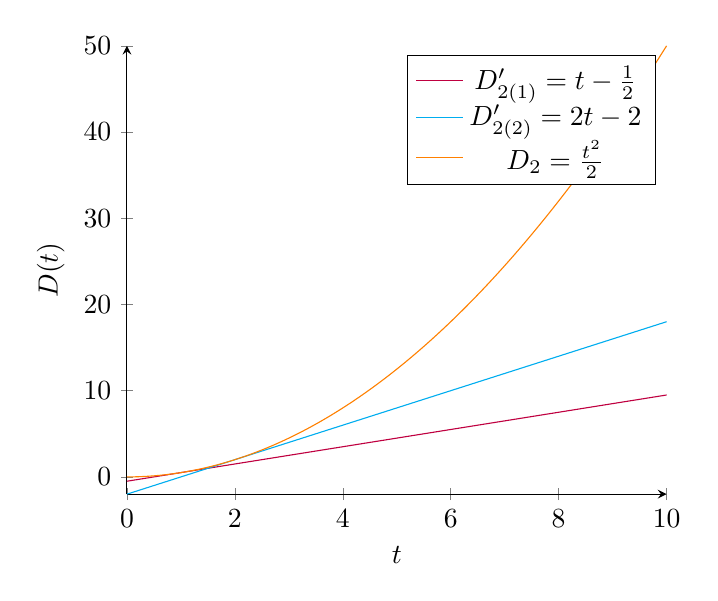
\begin{tikzpicture}
        \begin{axis}[
                axis lines = left,
                xlabel = \(t\),
                ylabel = {\(D(t)\)},
                clip = false,
            ]
            % D'_2 en 1
            \addplot [
                domain=0:10,
                samples=200,
                color=purple,
            ]
            {x-0.5};
            \addlegendentry{\(D'_{2(1)}=t-\frac{1}{2}\)}

            % D'_2 en 1
            \addplot [
                domain=0:10,
                samples=200,
                color=cyan,
            ]
            {2*x-2};
            \addlegendentry{\(D'_{2(2)}=2t-2\)}

            % D_2
            \addplot[
                domain=0:10,
                samples=200,
                color=orange,
            ]
            {x*x/2};
            \addlegendentry{\(D_2=\frac{t^2}{2}\)}
        \end{axis}
    \end{tikzpicture}
\end{center}

Las expresiones de las rectas tangentes se obtienen recurriendo a la notación punto-pendiente ($y-y_0 = m(x-x_0)$), despejando la $y$.

\vspace{10pt}

\textbf{f)} Como se desprende tanto de la tabla como de la representación gráfica, la velocidad del automóvil 1 es constante, mientras la del automóvil 2 se incrementa a medida que pasa el tiempo.
